\DiaryEntry{van der Pol Oscillator}{2024-09-24}{ODE}

\subsection{Introduction}

The ODE of the oscillator is given as

\be\label{20240924:eq1}
x'' - \mu(1-x^2)x' + x = x'' + \mu(x^2 - 1)x' + x = 0
\ee

We can convert this into an ODE system

\begin{align*}
y' &= \mu (1-x^2) y - x \\
x' &= y
\end{align*}

This is a special case of a Lienard System which is given by the following ODE,

\bee
x'' + f(x) x' + g(x) = 0
\eee

We can rewrite it as an ODE system

\begin{align*}
y' &= -g(x) - f(x)y \\
x' = y
\end{align*}

Setting  $f(x) = - \mu(1-x^2)$ and $g(x) = x$ yields the van der Pol oscillator. 

If the Lienard system fulfills certain criteria, it can be shown that the system has a unique, stable limit cycle surrounding the origin in the phase plane. The conditions are:

\begin{itemize}
\item $f(x)$ and $g(x)$ are continuously differentiable for all $x$
\item $g(x)$ is an odd function
\item $f(x)$ is an even function
\item The odd function $F(x) = \int_0^x f(u) du$ has exactly one positive zero at $x=a$, is negative for $0<x<a$, is positive and nondecreasing for $x>a$, and $F(x) \rightarrow \infty$ as $x \rightarrow \infty$.
\end{itemize}

This result should seem plausible. The assumptions on $g(x)$ mean that the restoring force acts like an ordinary spring, and tends to reduce any displacement, whereas the assumptions on $f(x)$ imply that the damping is negative at small $|x|$ and positive at large $|x|$. Since small oscillations are pumped up and large oscillations are damped down, it is not surprising that the system tends to settle into a self-sustained oscillation of some intermediate amplitude.

We can analyze the conditions for the van der Pol system with $f(x) = \mu(x^2 - 1)$ and $g(x) = x$. Conditions 1 - 4 are fulfilled, for the last we calculate

\bee
F(x) = \int_0^x f(u) du = \mu \left( \frac{x^3}{3} - x \right) = \frac{x^3}{3} \mu x (x^2 - 3)
\eee

This has one positive zero at $x = \sqrt{3}$, the last condition is fulfilled, and therefore the van der Pol system has a unique, stable limit cycle surrounding the origin in the phase plane.

\subsection{Relaxation Oscillations}

We consider the case $\mu >> 1$. In this strongly nonlinear limit, we will see that the limit cycle consists of an extremely slow buildup followed by a sudden discharge, followed by another slow buildup, and so on. Oscillations of this type are often called relaxation oscillations, because the “stress” accumulated during the slow buildup is “relaxed” during the sudden discharge. Relaxation oscillations occur in many other scientific contexts.

We start with introduction of new variables based on the observation,

\bee
x'' + \mu x' (x^2 - 1) = \frac{d}{dt} \left( x' + \mu \left[ \frac{1}{3} x^3 - x \right] \right)
\eee

We introduce $F(x) = \frac{1}{3} x^3 - x$ and $w = x' + \mu F(x)$ and then we have

\bee
x'' + \mu x' (x^2 - 1) = \frac{d}{dt} w
\eee

Going back to the van der Pol ODE \eqref{20240924:eq1}, we see that $x'' + \mu x' (x^2 - 1) = - x$ and therefore 

\bee
\frac{d}{dt} w = -x
\eee

Collecting everything together, we arrive at the following ODE system

\begin{align*}
x' &= w - \mu F(x) \\
w' &= -x
\end{align*}

One last substitution $y = w / \mu$ yields the new ODE system

\begin{align*}
x' &= \mu \left( y - F(x) \right) \\
y' &= - \frac{1}{\mu} x
\end{align*}

The nullclines are the key to understanding the motion. The trajectories zap horizontally onto the cubic nullcline $B \rightarrow C$. Then it crawls up the nullcline until it comes to the knee, point D. Afterwards it zaps over to the other branch of the cubic at A. This is followed by another crawl along the cubic until the trajectory reaches the next jumping-off point at A, and the motion continues periodically after that.

This analysis shows that the limit cycle has two widely separated time scales: one for the crawls $A \rightarrow B$ and $C \rightarrow D$ and the fast zaps $B \rightarrow C$ and $D \rightarrow A$.

With the above variable substitution, we can calculate an estimate for the oscillation period $T$ as two times the integral over $dt$ between time $t_A$ and $t_B$,

\bee
T \approx 2 \int_{t_A}^{t_B} dt
\eee

On the slow branches, we approximately have $x' \approx 0$ and therefore $y \approx F(x)$. Therefore

\bee
\frac{dy}{dt} \approx F'(x) \frac{dx}{dt} = (x^2 - 1) \frac{dx}{dt}
\eee

But from the ODE system, we have $y' = -x / \mu$ and therefore

\bee
\frac{dx}{dt} = \frac{dy}{dt} \frac{1}{x^2-1} = - \frac{x}{\mu(x^2-1)} \rightarrow dt = - \frac{\mu(x^2-1)}{x} dx
\eee

Note: Keep in mind that this is \emph{only} valid on the slow branches!

\begin{figure}[H]
    \centering
    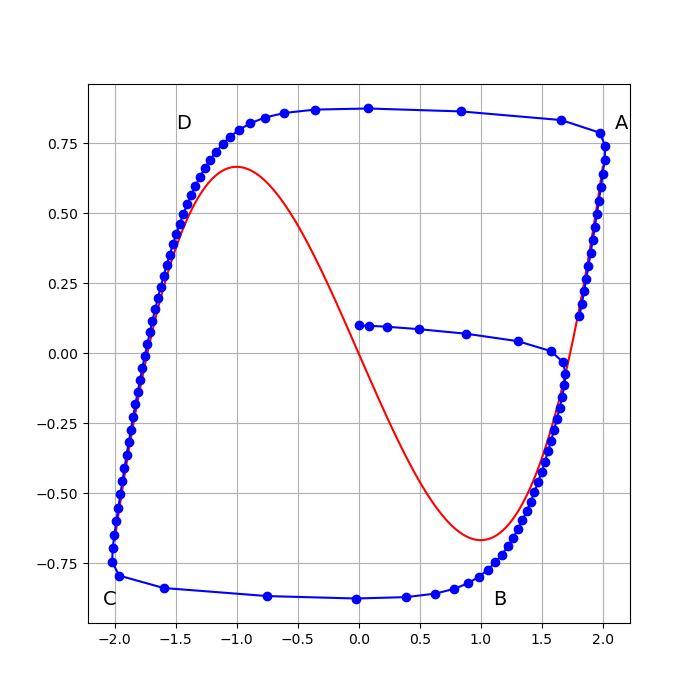
\includegraphics[scale=0.75]{images/2024-09-24-vanderpol_1.png}
\end{figure}

Before we can integrate, we need to know where the slow branch starts and ends; ie the coordinates $x_A, x_B$. Point B is given by the local minimum of $F(x)$,

\bee
\frac{dF(x)}{dx} = x^2 - 1 = 0 \rightarrow x = \pm 1
\eee

Looking at above Figure, we choose $x_B = 1$. By symmetry, $x_A = - x_C$ and from the Figure we take $y_B = y_C$. For $y_B$, we obtain $y_B = F(x_B) = -2/3$, and from this we get $x_A = 2$. So our integral finally becomes

\bee
T \approx - 2 \int_{x_B}^{x_A} \frac{\mu(x^2-1)}{x} dx = \cdots = \mu (3 - 2 \ln 2) \qed
\eee

\subsection{Weakly Nonliner Oscillators}

We consider oscillators with a small non-linear damping term,

\be\label{20240924:eq2}
x''  + x + \epsilon h(x, x') = 0
\ee

with $0 < \epsilon << 1$ and the smooth non-linear damping function $h(x, x')$. Setting $h(x, x') = (x^2-1)$ returns the van der Pol oscillator, $h(x, x') = x^3$ is the \emph{Duffing equation}.

The common theme of the solutions is that they exhibit two time scales: A slow one for the amplitude build-up and a fast one for the oscillations. There is an analytical method called \emph{two-timing} which produces good approximations for this behaviour, which we will use in the following.

To apply two-timing, let $\tau = t$ denote the fast time, and let $T = \epsilon t$ denote the slow time. We will treat these two times as if they were independent variables. In particular, functions of the slow time $T$ will be regarded as constants on the fast time scale $\tau$. It’s hard to justify this idea rigorously, but it works!

We start with a series expansion of \eqref{20240924:eq2},

\be\label{20240924:eq3}
x(t, \epsilon) = x_0(\tau, T) + \epsilon x_1(\tau, T) + \Oc(\epsilon^2)
\ee

The time derivatives can be obtained by means of the chain rule,

\bee
x' = \frac{dx}{dt} = \frac{\partial x}{\partial \tau} + \frac{\partial x}{\partial T} \frac{\partial T}{\partial t} = \frac{\partial x}{\partial \tau} + \epsilon \frac{\partial x}{\partial T}
\eee

Let's simplify notation by writing $\partial_\tau x = \frac{\partial x}{\partial \tau}$ so that we arrive at

\bee
x' = \frac{dx}{dt} = \partial_\tau x + \epsilon \partial_T x
\eee

Let's use this in the series expansion \eqref{20240924:eq3},

\be\label{20240924:eq10}
x' = \partial_\tau x_0 + \epsilon ( \partial_T x_0 + \partial_\tau x_1 ) + \Oc(\epsilon^2)
\ee

and

\be\label{20240924:eq11}
x'' = \partial_{\tau \tau} x_0 + \epsilon (\partial_{\tau \tau} x_1 + 2 \partial_{T \tau} x_0) + \Oc(\epsilon^2)
\ee

We will use this approach to solve the damped linear oscillator.

\paragraph{Damped Linear Oscillator.} We want to solve

\bee
x'' + 2 \epsilon x' + x = 0
\eee

with initial value conditions $x(0) = 0, x'(0) = 1$. Using \eqref{20240924:eq10} and \eqref{20240924:eq11} we get 

\bee
\partial_{\tau \tau} x_0 + \epsilon ( \partial_{\tau \tau} x_1  + 2 \partial_{T \tau} x_0) + 2 \epsilon \partial_\tau x_0 + x_0  + \epsilon x_1 + \Oc(\epsilon^2) = 0
\eee

Let's collect all powers of $\epsilon^0$ to get

\bee
\partial_{\tau \tau} x_0 + x_0 = 0
\eee

which is a simple linear oscillator having solutions of the form

\bee
x_0(\tau) = A \sin \tau + B \cos \tau
\eee

However, the interesting part is that the “constants” $A$ and $B$ are actually functions of the slow time $T$. Here we are invoking the above mentioned ideas that $\tau$ and $T$ should be regarded as independent variables, with functions of $T$ behaving like constants on the fast time scale $\tau$.

We can determine $A(T)$ and $B(T)$ by looking at the next order of $\epsilon$. This yields

\bee
\partial_{\tau \tau} x_1  + 2 \partial_{T \tau} x_0 + 2 \partial_\tau x_0 + x_1 = 0
\eee

Separating $x_0$ and $x_1$ terms, we obtain

\bee
\partial_{\tau \tau} x_1 + x_1 = - 2 ( \partial_{T \tau} x_0 + \partial_\tau x_0)
\eee

Now inserting $_0(\tau) = A \sin \tau + B \cos \tau$ we obtain

\bee
\partial_{\tau \tau} x_1 + x_1 = -2 (A' + A) \cos \tau + 2(B' + B) \sin \tau
\eee

This is again a second-order ODE but with sinusoidal driving force which will cause resonant behaviour. We want to avoid that and - with some handwaving - we set the coefficients to zero,

\begin{align*}
    A' + A &= 0 \\
    B' + B &= 0
\end{align*}

This yields the solutions

\be\label{20240924:eq20}
A(T) = A(0) e^{-T}, \quad B(T) = B(0) e^{-T}
\ee

As a last step, we use the initial value conditions to obtain $A(0), B(0)$: We have $x(0) = 0$ and from \eqref{20240924:eq3}, we have 

\bee
0 = x(0) = x_0(0,0) + \epsilon x_1(0,0) + \Oc(\epsilon^2)
\eee

From this follows $x_0(0,0) = x_1(0,0) = 0$. Inserting this into \eqref{20240924:eq20}, we find $B(0) = 0$.

Using the second initial value condition, $x'(0) = 1$ and \eqref{20240924:eq10}, we obtain

\bee
1 = x'(0) = \partial_\tau x_0(0,0) + \epsilon ( \partial_T x_0(0,0) + \partial_\tau x_1(0,0) ) + \Oc(\epsilon^2)
\eee

and therefore $\partial_\tau x_0(0,0) = 1$ and $\partial_T x_0(0,0) + \partial_\tau x_1(0,0) = 0$. Using $\partial_\tau x_0(0,0) = 1$ in \eqref{20240924:eq20}, we obtain $A(0) = 1$ and finally

\bee
x_0(\tau, T) = e^{-T} \sin \tau
\eee

For the final solution $x$ we have

\bee
x = e^{-T} \sin \tau + \Oc(\epsilon) = e^{-\epsilon t} \sin t + \Oc(epsilon) \qed
\eee

